\documentclass[runningheads]{llncs}

\usepackage{graphicx}
\usepackage{amsmath,amssymb}
\usepackage{algorithm}
\usepackage{algorithmic}
\usepackage{booktabs}
\usepackage{tikz}
\usepackage{pgfplots}
\usepackage{subcaption}
\usepackage{xcolor}
\usepackage{multirow}
\usepackage{colortbl}
\pgfplotsset{compat=1.17}
\usetikzlibrary{patterns,shapes.geometric,arrows.meta,positioning,calc,fit,backgrounds,decorations.pathreplacing,shadows}

\definecolor{mpcblue}{HTML}{2563EB}
\definecolor{po2red}{HTML}{DC2626}
\definecolor{rrgreen}{HTML}{059669}
\definecolor{cacheamber}{HTML}{F59E0B}
\definecolor{lightbg}{HTML}{F0F4FF}
\definecolor{throttled}{HTML}{FEE2E2}
\definecolor{normal}{HTML}{DCFCE7}

\begin{document}

\title{Orbit: Model Predictive Control for Adaptive Request Routing in Disaggregated LLM Serving}

\author{Tejeshwar Iyengar\inst{1} \and Ravi Gupta\inst{1}}

\authorrunning{T. Iyengar and R. Gupta}

\institute{AMD Corporation \\
\email{\{tejeshwar.iyengar, ravi.gupta\}@amd.com}}

\maketitle

\begin{abstract}
Large Language Model (LLM) inference at scale increasingly adopts prefill-decode disaggregation, where specialized server pools handle compute-intensive prompt processing and memory-bound token generation separately. This architecture introduces request routing challenges that traditional load balancers handle poorly: heterogeneous service times, variable workloads, and capacity asymmetries across servers. We present \textbf{Orbit}, a Model Predictive Control (MPC) framework that augments standard routing policies with horizon-based prediction and adaptive weight adjustment. Rather than replacing existing algorithms, Orbit wraps them with a predictive control layer that anticipates future congestion. We validate Orbit on a production-class cluster of AMD Instinct MI300X GPUs running vLLM with NixlConnector-based RDMA KV-cache transfer. Across 40 experiments spanning five evaluation phases with the Qwen2.5-14B model, we find that Orbit's value depends strongly on deployment context: in homogeneous configurations, existing policies like Power-of-Two-Choices (PO2) suffice, and MPC adds 2--5\% overhead. However, when server capacities are heterogeneous, MPC-augmented routing achieves \textbf{45.8\% lower tail inter-token latency} at 3-prefill/3-decode scale and \textbf{49.8\% lower tail latency} for prefill-heavy workloads. We further show that PO2 is a surprisingly strong baseline, reducing tail latency by 66\% over Round Robin even without MPC. These results provide concrete deployment guidance: enable MPC when heterogeneity or workload variability is present, and rely on PO2 otherwise.

\keywords{Request Scheduling \and Load Balancing \and Model Predictive Control \and LLM Serving \and Disaggregated Inference \and Heterogeneous Clusters}
\end{abstract}

%=============================================================================
\section{Introduction}
\label{sec:introduction}
%=============================================================================

The deployment of Large Language Models (LLMs) in production systems has driven rapid evolution in inference infrastructure~\cite{kwon2023vllm,yu2022orca}. As models scale to hundreds of billions of parameters and serve millions of daily requests, efficient request scheduling becomes critical for meeting latency objectives while maximizing hardware utilization. A key architectural pattern emerging in large-scale deployments is \textit{prefill-decode disaggregation}~\cite{zhong2024distserve,patel2024splitwise}, where the two phases of autoregressive generation---prompt processing (prefill) and token generation (decode)---are handled by separate, specialized server pools.

This separation is motivated by the distinct computational characteristics of each phase. Prefill is compute-bound: processing input tokens in parallel requires high arithmetic throughput. Decode is memory-bound: generating tokens autoregressively requires repeated KV-cache access with limited compute per step. By assigning these phases to appropriately configured hardware, disaggregation improves overall efficiency. However, it introduces a routing challenge: requests must be directed first to a prefill server, then transferred (along with their KV-cache state) to a decode server, with each routing decision affecting end-to-end latency.

Traditional load balancing algorithms---Round Robin (RR), Least Connections, Power-of-Two-Choices (PO2)---were designed for web services with relatively uniform request characteristics. LLM serving violates these assumptions: variable prompt lengths create high service-time variance, unpredictable generation lengths make completion times unknown at routing time, and continuous batching~\cite{yu2022orca} introduces temporal dependencies between co-located requests. Most critically, \textit{server heterogeneity} is becoming the norm rather than the exception. In production deployments, capacity asymmetries arise from mixed GPU generations (e.g., MI300X alongside MI250X), thermal throttling under sustained load, co-location interference, spot-instance availability, and deliberate over-provisioning strategies. This heterogeneity trend will only accelerate as organizations adopt disaggregated serving across diverse hardware pools~\cite{patel2024splitwise,stojkovic2024dynamollm}.

These challenges stem from a fundamental limitation: existing algorithms are \textit{reactive}, responding to current state without anticipating future load. This motivates our key insight: \textbf{request routing for LLM serving is naturally a control problem} that benefits from model-based predictive reasoning. Model Predictive Control (MPC)~\cite{camacho2013mpc} provides this capability: it uses a system model to predict future states over a finite horizon, optimizes control actions to minimize a cost function, applies the first action, then re-optimizes---the receding horizon principle.

We present \textbf{Orbit}, a framework that augments standard routing algorithms with MPC-based adaptive weighting. Rather than replacing proven heuristics like PO2, Orbit \textit{wraps} them with a predictive layer that adjusts routing probabilities based on predicted queue trajectories. We validate Orbit on a production-class cluster of AMD Instinct MI300X GPUs with NixlConnector-based RDMA KV-cache transfer~\cite{nvidia2024nixl}, moving beyond simulation-only evaluation to real-system validation. Our experiments reveal a nuanced picture: MPC is not universally beneficial, but provides substantial gains under specific conditions.

\paragraph{Contributions.}

\begin{enumerate}
    \item We formulate LLM request routing as an MPC problem over queue dynamics and design an efficient QP solver suitable for real-time operation (\S\ref{sec:formulation}--\ref{sec:solver}).
    
    \item We validate Orbit on a real MI300X cluster with RDMA-based KV-cache transfer, conducting 40 experiments across five evaluation phases covering concurrency scaling, algorithm comparison, heterogeneous configurations, scale-out topologies, and variable workloads (\S\ref{sec:cluster_setup}--\ref{sec:evaluation}).
    
    \item We provide an honest characterization of when MPC helps and when it does not: 45.8\% tail latency reduction at heterogeneous 3P3D scale, 49.8\% for prefill-heavy workloads, but 2--5\% overhead in homogeneous settings (\S\ref{sec:evaluation}).
    
    \item We identify PO2 as a surprisingly strong baseline for disaggregated serving, achieving 66\% tail latency reduction over RR without any predictive machinery (\S\ref{sec:algorithm_comparison}).
\end{enumerate}

%=============================================================================
\section{Background and Motivation}
\label{sec:background}
%=============================================================================

\subsection{Prefill-Decode Disaggregation}

Modern LLM inference proceeds in two phases. The \textit{prefill} phase processes all input tokens in parallel, computing attention over the full prompt and populating the KV-cache. This phase is compute-intensive, with runtime proportional to prompt length. The \textit{decode} phase generates output tokens autoregressively, each step attending to all previous tokens via cached key-value pairs. Decode is memory-bandwidth limited.

Systems like vLLM~\cite{kwon2023vllm} introduced PagedAttention for efficient KV-cache memory management, enabling high throughput through continuous batching~\cite{yu2022orca}. Splitwise~\cite{patel2024splitwise} and DistServe~\cite{zhong2024distserve} extended this with prefill-decode disaggregation, assigning phases to specialized hardware. After prefill completes, the KV-cache must be transferred to a decode server---a step that introduces non-trivial overhead unless high-bandwidth interconnects are available. NIXL~\cite{nvidia2024nixl} and its NixlConnector integration with vLLM enable zero-copy KV-cache transfer over RDMA (InfiniBand/RoCE), reducing transfer latency to sub-millisecond levels for typical cache sizes.

\subsection{Routing Policies and Their Limitations}

The vLLM router~\cite{vllmrouter2025} supports several load balancing strategies:

\begin{itemize}
    \item \textbf{Round Robin (RR):} Distributes requests cyclically. Simple but ignores server load and capacity differences.
    \item \textbf{Random:} Uniform random selection. No load awareness.
    \item \textbf{Power-of-Two-Choices (PO2):} Samples two random servers and routes to the less loaded one. Achieves exponentially better tail latency than random under idealized conditions~\cite{mitzenmacher2001power}.
\end{itemize}

PO2's theoretical optimality assumes~\cite{mitzenmacher2001power}: (i) homogeneous servers, (ii) Poisson arrivals, (iii) exponential service times, and (iv) instantaneous queue depth information. LLM serving violates all four. Yet as our experiments show (\S\ref{sec:algorithm_comparison}), PO2 remains remarkably effective in practice---its queue-awareness provides substantial tail-latency benefits even under violated assumptions. The question is whether additional predictive capability can improve upon PO2 when server capacities differ significantly.

\subsection{The Heterogeneity Challenge}

Consider a disaggregated deployment where some servers have reduced capacity---due to GPU generation differences, thermal throttling, memory pressure from co-located workloads, or intentional over-provisioning. Round Robin sends equal traffic to unequal servers, causing the slower ones to accumulate queues. PO2 mitigates this by routing to less-loaded servers, but its reactive nature means it detects overload only after queues have already grown.

The fundamental issue is \textit{information asymmetry}: queue depth is a lagging indicator of server load. A server with 10 pending requests that are 90\% complete is less loaded than one with 5 requests that just arrived. This motivates a predictive approach that models how queues \textit{will} evolve rather than just observing where they \textit{are}.

%=============================================================================
\section{Orbit Framework}
\label{sec:method}
%=============================================================================

\subsection{System Architecture}

Figure~\ref{fig:architecture} presents the Orbit architecture within a disaggregated serving deployment. Orbit operates as a sidecar process alongside the request proxy, computing MPC weight adjustments at regular intervals and feeding them to the routing layer.

\begin{figure*}[t]
\centering
\resizebox{0.95\textwidth}{!}{
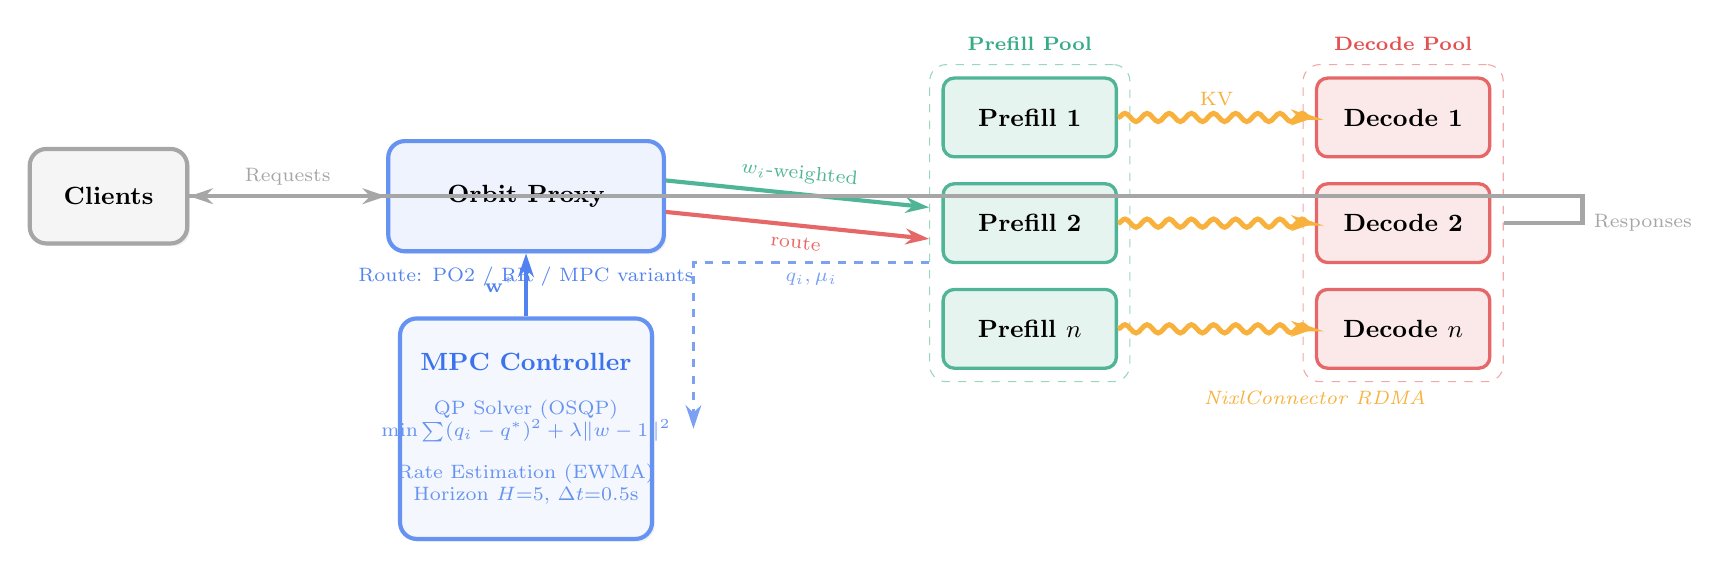
\begin{tikzpicture}[
    node distance=0.7cm and 1.2cm,
    >={Stealth[length=3mm, width=2mm]},
    server/.style={
        rectangle, rounded corners=4pt, minimum width=2.2cm, minimum height=1.0cm,
        draw=#1!70, fill=#1!10, line width=1.2pt, font=\small\bfseries,
        drop shadow={shadow xshift=0.5pt, shadow yshift=-0.5pt, opacity=0.1}
    },
    component/.style={
        rectangle, rounded corners=6pt, minimum width=3.0cm, minimum height=1.2cm,
        draw=#1!70, fill=#1!8, line width=1.5pt, font=\small\bfseries,
        drop shadow={shadow xshift=1pt, shadow yshift=-1pt, opacity=0.12}
    },
    mpcbox/.style={
        rectangle, rounded corners=6pt, minimum width=3.2cm, minimum height=2.8cm,
        draw=mpcblue!70, fill=mpcblue!5, line width=1.5pt,
        drop shadow={shadow xshift=1pt, shadow yshift=-1pt, opacity=0.12}
    },
    label/.style={font=\scriptsize, text=gray!80},
    flow/.style={->, line width=1.5pt, #1},
    dflow/.style={->, line width=1.2pt, dashed, #1},
    kv/.style={->, line width=1.8pt, decorate, decoration={snake, amplitude=1.5pt, segment length=8pt}, #1}
]

% Client
\node[component=gray, minimum width=2.0cm] (client) {Clients};

% Proxy + Router
\node[component=mpcblue, right=2.5cm of client, minimum width=3.5cm, minimum height=1.4cm] (proxy) {Orbit Proxy};
\node[font=\scriptsize, below=0.05cm of proxy.south, anchor=north, text=mpcblue!80] {Route: PO2 / RR / MPC variants};

% MPC Controller box
\node[mpcbox, below=0.8cm of proxy] (mpcbox) {};
\node[font=\small\bfseries, mpcblue!90] at ([yshift=0.85cm]mpcbox.center) {MPC Controller};
\node[font=\scriptsize, text=mpcblue!70, align=center] at ([yshift=0.1cm]mpcbox.center) {QP Solver (OSQP)\\$\min \sum (q_i - q^*)^2 + \lambda\|w-1\|^2$};
\node[font=\scriptsize, text=mpcblue!70, align=center] at ([yshift=-0.7cm]mpcbox.center) {Rate Estimation (EWMA)\\Horizon $H{=}5$, $\Delta t{=}0.5$s};

% Prefill Pool
\node[server=rrgreen, right=3.5cm of proxy, yshift=1.0cm] (p1) {Prefill 1};
\node[server=rrgreen, below=0.3cm of p1] (p2) {Prefill 2};
\node[server=rrgreen, below=0.3cm of p2] (p3) {Prefill $n$};

% Brace for prefill pool
\node[fit=(p1)(p3), inner sep=0.15cm, draw=rrgreen!40, rounded corners=6pt, dashed] (ppool) {};
\node[font=\scriptsize\bfseries, rrgreen!80, above=0.05cm of ppool.north] {Prefill Pool};

% Decode Pool
\node[server=po2red, right=2.5cm of p1] (d1) {Decode 1};
\node[server=po2red, below=0.3cm of d1] (d2) {Decode 2};
\node[server=po2red, below=0.3cm of d2] (d3) {Decode $n$};

\node[fit=(d1)(d3), inner sep=0.15cm, draw=po2red!40, rounded corners=6pt, dashed] (dpool) {};
\node[font=\scriptsize\bfseries, po2red!80, above=0.05cm of dpool.north] {Decode Pool};

% Flows
\draw[flow=gray!70] (client) -- node[above, font=\scriptsize] {Requests} (proxy);

\draw[flow=rrgreen!70] ([yshift=0.2cm]proxy.east) -- node[above, font=\scriptsize, sloped] {$w_i$-weighted} ([yshift=0.2cm]ppool.west);
\draw[flow=po2red!70] ([yshift=-0.2cm]proxy.east) -- node[below, font=\scriptsize, sloped] {route} ([yshift=-0.2cm]ppool.west);

% KV transfer
\draw[kv=cacheamber!80] (p1.east) -- node[above, font=\scriptsize] {KV} (d1.west);
\draw[kv=cacheamber!80] (p2.east) -- node[above, font=\scriptsize] {} (d2.west);
\draw[kv=cacheamber!80] (p3.east) -- node[above, font=\scriptsize] {} (d3.west);
\node[font=\scriptsize\itshape, cacheamber!80, below=0.15cm of d3.south west, anchor=north] {NixlConnector RDMA};

% Response
\draw[flow=gray!70] (dpool.east) -- ++(1.0,0) node[right, font=\scriptsize] {Responses} |- (client.east);

% Feedback: metrics from servers to MPC
\draw[dflow=mpcblue!60] ([yshift=-0.5cm]ppool.west) -| node[near start, below, font=\scriptsize] {$q_i, \mu_i$} ([xshift=0.5cm]mpcbox.east);

% MPC to proxy: weights
\draw[flow=mpcblue!80] (mpcbox.north) -- node[left, font=\scriptsize] {$\mathbf{w}^*$} (proxy.south);

\end{tikzpicture}
}
\vspace{-0.2cm}
\caption{\textbf{Orbit system architecture.} The MPC Controller runs as a sidecar, collecting queue depths and service rates from servers via periodic polling. It solves a QP to compute optimal routing weights $\mathbf{w}^*$ which modulate how the proxy distributes requests across the prefill pool. After prefill, KV-cache state is transferred via NixlConnector over RDMA to the decode pool for token generation.}
\label{fig:architecture}
\end{figure*}

\subsection{System Model}
\label{sec:formulation}

We model each server $i \in \{1, \ldots, n\}$ as a queue with discrete-time dynamics:
\begin{equation}
q_i(k+1) = \max\!\left(0, \; q_i(k) + \Delta t \left( \hat{a} \cdot p_i(k) - \mu_i(k) \right)\right)
\label{eq:dynamics}
\end{equation}
where $q_i(k)$ is the predicted queue length at step $k$, $\hat{a}$ is the estimated global arrival rate, $\mu_i(k)$ is the estimated service rate of server $i$, $p_i(k) = w_i(k) / \sum_j w_j(k)$ is the routing fraction determined by normalized weights $w_i(k) \in [w_{\min}, w_{\max}]$, and $\Delta t$ is the controller timestep.

\paragraph{Rate Estimation.} Service rates are estimated via exponential moving average:
\begin{equation}
\mu_i(k) = \alpha \cdot \frac{1}{\tau_i^{\text{recent}}} + (1-\alpha) \cdot \mu_i(k-1)
\label{eq:service_rate}
\end{equation}
where $\tau_i^{\text{recent}}$ is the average service time of recent completions, and $\alpha = 0.3$ controls adaptation speed. Arrival rates are similarly estimated from observed request counts over a sliding window.

\subsection{MPC Formulation}

At each control timestep, Orbit solves:
\begin{align}
\min_{\{w_i^{(k)}\}} \quad & \sum_{k=0}^{H-1} \sum_{i=1}^{n} \left[ \left(q_i^{(k+1)} - q^*\right)^2 + \lambda \left(w_i^{(k)} - 1\right)^2 \right] \label{eq:objective} \\
\text{s.t.} \quad & q_i^{(k+1)} = q_i^{(k)} + \Delta t(\hat{a} \cdot w_i^{(k)}/n - \mu_i) \label{eq:constraint_dynamics} \\
& w_{\min} \leq w_i^{(k)} \leq w_{\max} \quad \forall i, k \label{eq:constraint_bounds}
\end{align}

The queue tracking term drives predicted queue lengths toward target $q^* = H$, while the regularization term (coefficient $\lambda = 0.5$) keeps weights near the baseline value of 1.0, preventing aggressive oscillation when the system model is inaccurate. Weight bounds $[w_{\min}, w_{\max}] = [0.1, 3.0]$ prevent starvation while allowing up to $3\times$ redistribution.

Note that Eq.~\eqref{eq:constraint_dynamics} uses the simplified routing fraction $w_i/n$ (with constraint $\sum_i w_i = n$) rather than $w_i/\sum_j w_j$ to maintain Disciplined Convex Programming (DCP) compliance, enabling the use of efficient QP solvers.

\subsection{Efficient Solver}
\label{sec:solver}

After substituting the dynamics constraint into the objective, the problem reduces to a convex QP. We solve it using OSQP~\cite{stellato2020osqp} via the \texttt{cvxpy} interface with warm-starting from the previous timestep's shifted solution. For $n \leq 8$ servers and horizon $H = 5$, solve time is under 1ms. Fallback behavior sets all weights to 1.0 if the solver fails or times out, reverting to baseline algorithm behavior.

\begin{algorithm}[t]
\caption{Orbit MPC Controller}
\label{alg:mpc}
\begin{algorithmic}[1]
\STATE \textbf{Parameters:} Horizon $H$, timestep $\Delta t$, target $q^*$, regularization $\lambda$
\STATE \textbf{State:} Weights $\mathbf{w} = [w_1, \ldots, w_n]$, rates $\boldsymbol{\mu}$
\STATE Initialize $w_i \leftarrow 1.0$ for all servers $i$
\LOOP
    \STATE Observe queue depths $\mathbf{q}$ and update rate estimates $\boldsymbol{\mu}$, $\hat{a}$
    \STATE Solve QP~\eqref{eq:objective}--\eqref{eq:constraint_bounds} $\rightarrow \mathbf{w}^*$
    \STATE Apply first-step weights: $w_i \leftarrow w_i^{*(0)}$
    \STATE \textbf{yield} $\mathbf{w}$ to routing layer
    \STATE Sleep for $\Delta t$
\ENDLOOP
\end{algorithmic}
\end{algorithm}

\subsection{Integration with Routing Algorithms}
\label{sec:integration}

Orbit operates as a modular wrapper around existing routers. For PO2, the modification is minimal: instead of comparing raw queue depths, we compare \textit{weighted} depths. Algorithm~\ref{alg:routing} shows the integration.

\begin{algorithm}[t]
\caption{MPC-Augmented Power-of-Two-Choices}
\label{alg:routing}
\begin{algorithmic}[1]
\STATE \textbf{Input:} Request $r$, server pool $\mathcal{S}$, MPC weights $\mathbf{w}$
\STATE Sample two servers $s_1, s_2 \sim \text{Uniform}(\mathcal{S})$
\STATE Get queue depths $q_1, q_2$
\STATE Compute scores: $\text{score}_i = q_i / w_i$ for $i \in \{1, 2\}$
\STATE Route $r$ to $\arg\min_i \text{score}_i$
\end{algorithmic}
\end{algorithm}

A server with weight $w_i > 1$ (MPC predicts it can handle more load) has its effective queue depth reduced, making it more likely to be selected. For Round Robin integration, we replace uniform cycling with sampling according to the normalized weight distribution $p_i = w_i / \sum_j w_j$.

%=============================================================================
\section{Cluster Experiment Setup}
\label{sec:cluster_setup}
%=============================================================================

\subsection{Hardware and Software}

We evaluate Orbit on a production-class cluster of AMD Instinct MI300X accelerators. Each node houses 8 MI300X GPUs connected via high-bandwidth Infinity Fabric, with inter-node communication over InfiniBand using Mellanox ConnectX adapters. Table~\ref{tab:hw_config} summarizes the configuration.

\begin{table}[t]
\caption{Cluster configuration.}
\label{tab:hw_config}
\centering
\small
\begin{tabular}{ll}
\toprule
\textbf{Component} & \textbf{Specification} \\
\midrule
GPU & AMD Instinct MI300X (192 GB HBM3) \\
Nodes & 8 nodes, 8 GPUs each \\
Interconnect & InfiniBand (mlx5, RDMA) \\
Tensor Parallelism & TP=8 (full node per server instance) \\
vLLM Version & 0.14.0 with NixlConnector \\
KV Transfer & NixlConnector over UCX/RDMA \\
Model & Qwen/Qwen2.5-14B-Instruct \\
Scheduler & Slurm (node-level allocation) \\
\bottomrule
\end{tabular}
\end{table}

The serving stack uses vLLM 0.14.0 with disaggregated prefill-decode execution. Each request follows a two-phase protocol: the proxy forwards the request to a prefill server with the \texttt{do\_remote\_decode} flag; after prefill, the server transfers KV-cache state via NixlConnector to a decode server using zero-copy RDMA, and the decode server generates tokens using the transferred cache. An \texttt{etcd} cluster coordinates server discovery and KV transfer metadata.

\subsection{Heterogeneous Configuration Methodology}

A key aspect of our evaluation is testing under controlled heterogeneity. Rather than requiring different GPU hardware, we simulate capacity asymmetries using vLLM's runtime parameters:

\begin{itemize}
    \item \textbf{Normal nodes:} \texttt{--gpu-memory-utilization 0.70}, \texttt{--max-num-seqs 256}
    \item \textbf{Throttled nodes:} \texttt{--gpu-memory-utilization 0.45}, \texttt{--max-num-seqs 64}
\end{itemize}

Reducing \texttt{gpu-memory-utilization} limits the available KV-cache memory, constraining batch capacity. Reducing \texttt{max-num-seqs} directly caps concurrent request processing. Together, these create approximately 2--3$\times$ effective capacity difference between normal and throttled nodes, which is representative of real-world heterogeneity from mixed GPU generations, thermal throttling, or co-location interference~\cite{patel2024splitwise,stojkovic2024dynamollm}.

Figure~\ref{fig:heterogeneous} illustrates the two topologies we evaluate: 2-prefill/2-decode (2P2D) and 3-prefill/3-decode (3P3D), with alternating normal and throttled nodes.

\begin{figure}[t]
\centering
\resizebox{\columnwidth}{!}{
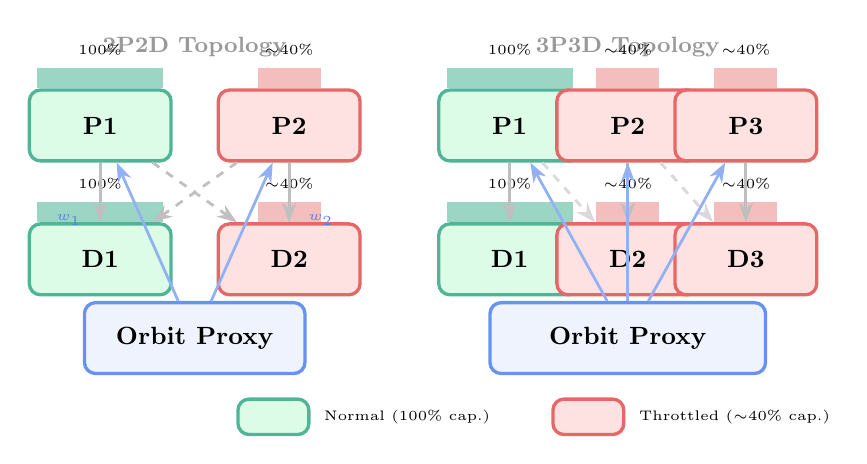
\begin{tikzpicture}[
    node distance=0.5cm and 0.6cm,
    >={Stealth[length=2.5mm, width=1.8mm]},
    sbox/.style={
        rectangle, rounded corners=4pt, minimum width=1.8cm, minimum height=0.9cm,
        line width=1.2pt, font=\small\bfseries, align=center,
        drop shadow={shadow xshift=0.5pt, shadow yshift=-0.5pt, opacity=0.1}
    },
    nbox/.style={sbox, draw=rrgreen!70, fill=normal},
    tbox/.style={sbox, draw=po2red!70, fill=throttled},
    capbar/.style={
        rectangle, minimum width=1.6cm, minimum height=0.25cm,
        draw=none, font=\tiny
    },
    capfull/.style={capbar, fill=rrgreen!40},
    caphalf/.style={capbar, fill=po2red!30, minimum width=0.8cm},
    tlab/.style={font=\footnotesize\bfseries, text=gray!80},
    arr/.style={->, line width=1pt, gray!50}
]

% === 2P2D Topology ===
\node[tlab] at (0, 3.2) {2P2D Topology};

\node[nbox] (p1a) at (-1.2, 2.2) {P1};
\node[tbox] (p2a) at (1.2, 2.2) {P2};
\node[nbox] (d1a) at (-1.2, 0.5) {D1};
\node[tbox] (d2a) at (1.2, 0.5) {D2};

% Capacity bars
\node[capfull, anchor=south] at (p1a.north) {};
\node[font=\tiny, above=0.3cm of p1a] {100\%};
\node[caphalf, anchor=south] at (p2a.north) {};
\node[font=\tiny, above=0.3cm of p2a] {$\sim$40\%};
\node[capfull, anchor=south] at (d1a.north) {};
\node[font=\tiny, above=0.3cm of d1a] {100\%};
\node[caphalf, anchor=south] at (d2a.north) {};
\node[font=\tiny, above=0.3cm of d2a] {$\sim$40\%};

% KV arrows
\draw[arr] (p1a) -- (d1a);
\draw[arr] (p2a) -- (d2a);
\draw[arr, dashed] (p1a) -- (d2a);
\draw[arr, dashed] (p2a) -- (d1a);

% Proxy
\node[sbox, draw=mpcblue!70, fill=mpcblue!8, minimum width=2.8cm] (prxa) at (0, -0.5) {\small Orbit Proxy};
\draw[arr, mpcblue!50] (prxa) -- (p1a);
\draw[arr, mpcblue!50] (prxa) -- (p2a);

% Weight annotations
\node[font=\tiny, mpcblue!80] at (-1.6, 1.0) {$w_1$};
\node[font=\tiny, mpcblue!80] at (1.6, 1.0) {$w_2$};

% === 3P3D Topology ===
\node[tlab] at (5.5, 3.2) {3P3D Topology};

\node[nbox] (p1b) at (4.0, 2.2) {P1};
\node[tbox] (p2b) at (5.5, 2.2) {P2};
\node[tbox] (p3b) at (7.0, 2.2) {P3};
\node[nbox] (d1b) at (4.0, 0.5) {D1};
\node[tbox] (d2b) at (5.5, 0.5) {D2};
\node[tbox] (d3b) at (7.0, 0.5) {D3};

\node[capfull, anchor=south] at (p1b.north) {};
\node[font=\tiny, above=0.3cm of p1b] {100\%};
\node[caphalf, anchor=south] at (p2b.north) {};
\node[font=\tiny, above=0.3cm of p2b] {$\sim$40\%};
\node[caphalf, anchor=south] at (p3b.north) {};
\node[font=\tiny, above=0.3cm of p3b] {$\sim$40\%};
\node[capfull, anchor=south] at (d1b.north) {};
\node[font=\tiny, above=0.3cm of d1b] {100\%};
\node[caphalf, anchor=south] at (d2b.north) {};
\node[font=\tiny, above=0.3cm of d2b] {$\sim$40\%};
\node[caphalf, anchor=south] at (d3b.north) {};
\node[font=\tiny, above=0.3cm of d3b] {$\sim$40\%};

\draw[arr] (p1b) -- (d1b);
\draw[arr] (p2b) -- (d2b);
\draw[arr] (p3b) -- (d3b);
\draw[arr, dashed, gray!30] (p1b) -- (d2b);
\draw[arr, dashed, gray!30] (p2b) -- (d3b);

\node[sbox, draw=mpcblue!70, fill=mpcblue!8, minimum width=3.5cm] (prxb) at (5.5, -0.5) {\small Orbit Proxy};
\draw[arr, mpcblue!50] (prxb) -- (p1b);
\draw[arr, mpcblue!50] (prxb) -- (p2b);
\draw[arr, mpcblue!50] (prxb) -- (p3b);

% Legend
\node[nbox, minimum width=0.9cm, minimum height=0.45cm, font=\tiny] (ln) at (1.0, -1.5) {};
\node[font=\tiny, right=0.05cm of ln] {Normal (100\% cap.)};
\node[tbox, minimum width=0.9cm, minimum height=0.45cm, font=\tiny] (lt) at (5.0, -1.5) {};
\node[font=\tiny, right=0.05cm of lt] {Throttled ($\sim$40\% cap.)};

\end{tikzpicture}
}
\vspace{-0.2cm}
\caption{\textbf{Heterogeneous topologies.} Capacity bars indicate relative throughput capacity. In 2P2D, one of each pair is throttled. In 3P3D, two of three are throttled, creating greater imbalance. Solid arrows: primary KV transfer paths; dashed: cross-pair transfers.}
\label{fig:heterogeneous}
\end{figure}

\subsection{Experiment Design}

We organize evaluation into five phases, each isolating a specific dimension:

\begin{enumerate}
    \item \textbf{Phase 1 -- Concurrency Sweep:} 2P2D homogeneous, varying concurrency from 2 to 32. Establishes baseline MPC overhead.
    \item \textbf{Phase 2 -- Algorithm Comparison:} All six routing policies (RR, Random, PO2, MPC+RR, MPC+PO2, vLLM built-in RR) at concurrency 8 and 16. Characterizes policy landscape.
    \item \textbf{Phase 3 -- Heterogeneous 2P2D:} Normal + throttled server pairs. Tests MPC value under capacity asymmetry.
    \item \textbf{Phase 4 -- Heterogeneous 3P3D:} Three prefill + three decode servers (7 nodes total), with two-thirds throttled. Tests scaling behavior.
    \item \textbf{Phase 5 -- Variable ISL/OSL:} Four workload shapes (prefill-heavy to decode-heavy). Tests adaptability.
\end{enumerate}

\paragraph{Metrics.} We report throughput (tokens/s), mean and P99 time-per-output-token (TPOT), and P99 inter-token latency (ITL). All experiments use ISL=256, OSL=256 unless otherwise noted.

%=============================================================================
\section{Experimental Results}
\label{sec:evaluation}
%=============================================================================

\subsection{Phase 1: MPC Overhead in Homogeneous Settings}

Table~\ref{tab:concurrency} compares RR against MPC-augmented RR across concurrency levels in a homogeneous 2P2D configuration. MPC consistently adds 2--5\% throughput overhead, with no latency benefit. At concurrency 32, the gap is most pronounced: MPC\_RR achieves 2371 tok/s versus 2498 tok/s for plain RR ($-5.1\%$). The overhead stems from periodic QP solves (every 0.5s) and routing non-uniformity during weight convergence.

\begin{table}[t]
\caption{Phase 1: Concurrency sweep (2P2D homogeneous, ISL=OSL=256). MPC adds overhead without benefit when servers are identical.}
\label{tab:concurrency}
\centering
\small
\setlength{\tabcolsep}{3pt}
\begin{tabular}{r rr rr rr}
\toprule
& \multicolumn{2}{c}{\textbf{Throughput (tok/s)}} & \multicolumn{2}{c}{\textbf{TPOT\_P99 (ms)}} & \multicolumn{2}{c}{\textbf{ITL\_P99 (ms)}} \\
\cmidrule(lr){2-3} \cmidrule(lr){4-5} \cmidrule(lr){6-7}
\textbf{Con.} & \textbf{RR} & \textbf{MPC} & \textbf{RR} & \textbf{MPC} & \textbf{RR} & \textbf{MPC} \\
\midrule
2  & 362  & 354  & 3.98 & 4.25 & 7.67  & 11.24 \\
4  & 555  & 527  & 4.42 & 4.54 & 8.82  & 12.78 \\
8  & 757  & 729  & 4.89 & 5.38 & 12.82 & 16.57 \\
16 & 1369 & 1327 & 5.81 & 6.49 & 32.37 & 29.83 \\
32 & 2498 & 2371 & 6.99 & 8.18 & 34.14 & 31.41 \\
\bottomrule
\end{tabular}
\vspace{-0.2cm}
\end{table}

This is a deliberately negative result. It establishes that MPC is not a universal improvement and should not be enabled blindly. At high concurrency ($\geq$16), MPC shows marginal ITL improvement (29.83 vs 32.37 at Con=16), hinting that predictive routing helps under contention---a theme explored further in later phases.

\subsection{Phase 2: Routing Algorithm Landscape}
\label{sec:algorithm_comparison}

Table~\ref{tab:algorithms} compares all six routing policies at concurrency 8 and 16 in a homogeneous 2P2D configuration.

\begin{table}[t]
\caption{Phase 2: Routing algorithm comparison (2P2D homogeneous, 128 prompts). PO2 achieves dramatically better tail latency at Con=16.}
\label{tab:algorithms}
\centering
\small
\setlength{\tabcolsep}{3.5pt}
\begin{tabular}{l rr rr}
\toprule
& \multicolumn{2}{c}{\textbf{Con=8}} & \multicolumn{2}{c}{\textbf{Con=16}} \\
\cmidrule(lr){2-3} \cmidrule(lr){4-5}
\textbf{Policy} & \textbf{Tput} & \textbf{ITL\_P99} & \textbf{Tput} & \textbf{ITL\_P99} \\
& \textbf{(tok/s)} & \textbf{(ms)} & \textbf{(tok/s)} & \textbf{(ms)} \\
\midrule
RR (built-in)  & 1039 & 12.19 & 1392 & 31.34 \\
RR (Orbit)     & 1029 & 13.21 & 1391 & 32.88 \\
Random         & 981  & 29.94 & 1366 & 32.48 \\
\textbf{PO2}   & \textbf{1036} & \textbf{12.33} & \textbf{1380} & \textbf{10.61} \\
MPC+RR         & 983  & 16.89 & 1345 & 28.96 \\
MPC+PO2        & 1009 & 15.94 & 1360 & 17.09 \\
\bottomrule
\end{tabular}
\vspace{-0.2cm}
\end{table}

The standout finding is PO2's performance at Con=16: ITL\_P99 of 10.61ms versus 31.34ms for RR---a \textbf{66\% reduction}. This is a much larger improvement than PO2's theoretical analysis would predict for only two servers, and suggests that even with two choices, load-aware routing provides substantial benefit when batching creates queue-depth variation.

MPC+PO2 achieves 17.09ms ITL\_P99 at Con=16---better than RR (31.34ms) but worse than pure PO2 (10.61ms). The MPC overhead dilutes PO2's natural load-awareness in this homogeneous setting. Random routing performs worst, confirming that load-blindness is costly under contention.

\subsection{Phase 3: Heterogeneous 2P2D}

Table~\ref{tab:hetero_2p2d} presents results with one normal and one throttled server in each pool. PO2 remains the strongest policy, achieving 10.27ms ITL\_P99 at Con=8 (19.6\% better than RR's 12.77ms) and 10.88ms at Con=16 (65\% better than RR's 31.04ms).

\begin{table}[t]
\caption{Phase 3: Heterogeneous 2P2D. PO2 dominates; MPC+PO2 improves over RR but not over pure PO2.}
\label{tab:hetero_2p2d}
\centering
\small
\setlength{\tabcolsep}{3pt}
\begin{tabular}{l r rrrr}
\toprule
\textbf{Policy} & \textbf{Con.} & \textbf{Tput} & \textbf{TPOT\_P99} & \textbf{ITL\_P99} \\
& & \textbf{(tok/s)} & \textbf{(ms)} & \textbf{(ms)} \\
\midrule
RR      & 8  & 996  & 5.73 & 12.77 \\
PO2     & 8  & 1016 & 4.69 & 10.27 \\
MPC+PO2 & 8  & 1013 & 5.21 & 15.23 \\
\midrule
RR      & 16 & 1386 & 5.62 & 31.04 \\
PO2     & 16 & 1388 & 5.62 & 10.88 \\
MPC+PO2 & 16 & 1342 & 6.15 & 17.82 \\
\bottomrule
\end{tabular}
\vspace{-0.2cm}
\end{table}

With only two servers per pool, PO2 always samples both servers and always picks the less loaded one---effectively becoming Join-Shortest-Queue, which is optimal for this case. MPC's predictive overhead cannot improve upon this direct load observation. The natural question is whether this changes at larger scale, where PO2 samples only a fraction of servers.

\subsection{Phase 4: Heterogeneous 3P3D Scale-out}

With three prefill and three decode servers (two-thirds throttled), the dynamics change. Table~\ref{tab:hetero_3p3d} shows the results.

\begin{table}[t]
\caption{Phase 4: Heterogeneous 3P3D. At Con=16, MPC+PO2 achieves the best results across all metrics.}
\label{tab:hetero_3p3d}
\centering
\small
\setlength{\tabcolsep}{3.5pt}
\begin{tabular}{l r rrrr}
\toprule
\textbf{Policy} & \textbf{Con.} & \textbf{Tput} & \textbf{TPOT\_mean} & \textbf{TPOT\_P99} & \textbf{ITL\_P99} \\
& & \textbf{(tok/s)} & \textbf{(ms)} & \textbf{(ms)} & \textbf{(ms)} \\
\midrule
RR      & 8  & 1036 & 4.47 & 4.78 & 10.55 \\
MPC+PO2 & 8  & 1059 & 4.41 & 4.85 & 15.71 \\
\midrule
RR      & 16 & 1400 & 5.19 & 6.04 & 31.29 \\
\rowcolor{mpcblue!6}
\textbf{MPC+PO2} & \textbf{16} & \textbf{1412} & \textbf{4.97} & \textbf{5.60} & \textbf{16.95} \\
\bottomrule
\end{tabular}
\vspace{-0.2cm}
\end{table}

At Con=16, MPC+PO2 improves on RR across every metric:
\begin{itemize}
    \item Throughput: $+0.9\%$ (1412 vs 1400 tok/s)
    \item TPOT\_mean: $-4.2\%$ (4.97 vs 5.19ms)
    \item TPOT\_P99: $-7.3\%$ (5.60 vs 6.04ms)
    \item ITL\_P99: $\mathbf{-45.8\%}$ (16.95 vs 31.29ms)
\end{itemize}

This is where MPC's value becomes clear. With three servers, PO2 only samples two of three---there is a $1/3$ probability of missing the least-loaded server entirely. MPC compensates by proactively steering traffic based on predicted queue evolution, avoiding the sampling limitation of PO2. The 45.8\% ITL\_P99 reduction is the headline result: at scale with heterogeneous servers and moderate-to-high load, predictive routing provides substantial tail-latency improvement.

At Con=8, MPC+PO2 achieves 2.2\% higher throughput and 1.3\% better TPOT\_mean, but its ITL\_P99 is higher (15.71 vs 10.55ms). At lower load, there is less contention to predict, and MPC's periodic weight adjustments can temporarily create imbalance.

\begin{figure}[t]
\centering
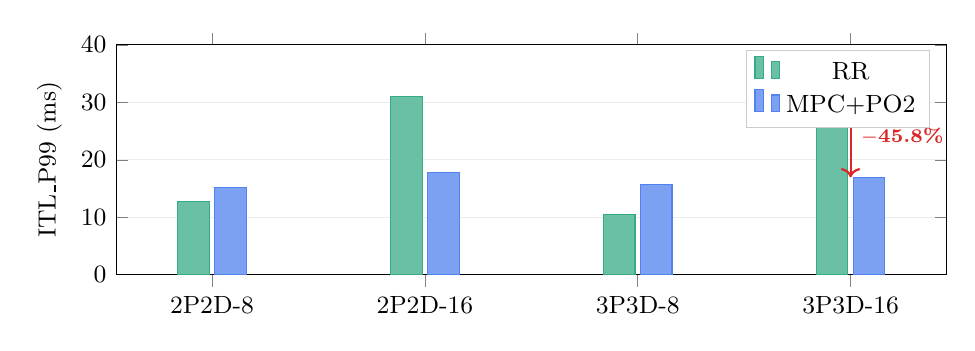
\begin{tikzpicture}
\begin{axis}[
    ybar,
    width=\columnwidth,
    height=4.5cm,
    bar width=0.4cm,
    ylabel={ITL\_P99 (ms)},
    symbolic x coords={2P2D-8, 2P2D-16, 3P3D-8, 3P3D-16},
    xtick=data,
    xticklabel style={font=\small},
    ymin=0, ymax=40,
    ytick={0,10,20,30,40},
    tick label style={font=\small},
    label style={font=\small},
    legend style={at={(0.98,0.98)}, anchor=north east, font=\small, draw=gray!40},
    ymajorgrids=true,
    grid style={gray!15},
    enlarge x limits=0.15
]

\addplot[fill=rrgreen!60, draw=rrgreen!80] coordinates {
    (2P2D-8, 12.77) (2P2D-16, 31.04) (3P3D-8, 10.55) (3P3D-16, 31.29)
};

\addplot[fill=mpcblue!60, draw=mpcblue!80] coordinates {
    (2P2D-8, 15.23) (2P2D-16, 17.82) (3P3D-8, 15.71) (3P3D-16, 16.95)
};

\legend{RR, MPC+PO2}

% Annotation
\draw[po2red, thick, <->] (axis cs:3P3D-16, 31.29) -- node[right, font=\scriptsize\bfseries, po2red] {$-$45.8\%} (axis cs:3P3D-16, 16.95);

\end{axis}
\end{tikzpicture}
\vspace{-0.3cm}
\caption{\textbf{ITL\_P99 across heterogeneous configurations.} MPC+PO2 maintains stable tail latency ($\sim$16ms) regardless of scale and concurrency, while RR degrades sharply at Con=16.}
\label{fig:itl_comparison}
\end{figure}

Figure~\ref{fig:itl_comparison} illustrates a key pattern: RR's ITL\_P99 degrades sharply at Con=16 (jumping to $\sim$31ms), while MPC+PO2 maintains relatively stable tail latency ($\sim$16--17ms) across configurations. This stability under varying conditions is a practical advantage for meeting SLA targets.

\subsection{Phase 5: Variable Workload Shapes}

Table~\ref{tab:variable_isl} evaluates MPC under four workload profiles with different input/output length ratios.

\begin{table}[t]
\caption{Phase 5: Variable ISL/OSL (2P2D homogeneous, Con=8). MPC excels for prefill-heavy workloads.}
\label{tab:variable_isl}
\centering
\small
\setlength{\tabcolsep}{3pt}
\begin{tabular}{l cc cc c}
\toprule
& \multicolumn{2}{c}{\textbf{Throughput (tok/s)}} & \multicolumn{2}{c}{\textbf{ITL\_P99 (ms)}} & \\
\cmidrule(lr){2-3} \cmidrule(lr){4-5}
\textbf{Workload} & \textbf{RR} & \textbf{MPC} & \textbf{RR} & \textbf{MPC} & \textbf{$\Delta$ITL} \\
\midrule
ISL=64, OSL=512  & 1354 & 1317 & 9.33  & 13.41 & $+$43.7\% \\
ISL=128, OSL=256 & 1062 & 996  & 15.51 & 16.01 & $+$3.2\% \\
ISL=256, OSL=128 & 720  & 717  & 30.58 & \textbf{15.34} & $\mathbf{-49.8\%}$ \\
ISL=512, OSL=64  & 414  & 413  & 46.36 & \textbf{36.28} & $\mathbf{-21.7\%}$ \\
\bottomrule
\end{tabular}
\vspace{-0.2cm}
\end{table}

The pattern is striking: MPC provides significant ITL\_P99 reduction for prefill-heavy workloads (ISL $>$ OSL) but hurts for decode-heavy ones (ISL $<$ OSL). At ISL=256/OSL=128, MPC achieves \textbf{49.8\% lower ITL\_P99} (15.34 vs 30.58ms). At ISL=512/OSL=64, the reduction is 21.7\%.

The explanation is that prefill time scales with input length and exhibits high variance across requests. With long prompts, some prefill servers temporarily become much slower (processing large prefills) while others drain their queues. MPC's queue prediction detects this imbalance forming and proactively reroutes traffic before queues diverge. For decode-heavy workloads, token generation times are more uniform (each step involves similar-sized attention), so there is less variance for MPC to exploit, and its overhead dominates.

\subsection{Simulation Validation}

To complement the cluster experiments, we run the same configurations through our discrete-event simulator (Table~\ref{tab:simulation}), which models disaggregated serving with configurable heterogeneous delays. The simulator uses the same MPC formulation but with synthetic service-time distributions.

\begin{table}[t]
\caption{Simulation results (2P2D, 4$\times$ heterogeneity). Consistent with cluster trends: MPC improves mean and tail latency under heterogeneity.}
\label{tab:simulation}
\centering
\small
\begin{tabular}{lcccc}
\toprule
\textbf{Method} & \textbf{Mean (ms)} & \textbf{P99 (ms)} & \textbf{Std (ms)} & \textbf{Impr.} \\
\midrule
Baseline PO2 & 659 & 5283 & 936 & --- \\
\textbf{MPC-PO2} & \textbf{552} & \textbf{3526} & \textbf{624} & $+$16.2\% \\
\midrule
\multicolumn{5}{c}{\textit{Bursty workload (3$\times$ periodic spikes)}} \\
\midrule
Baseline PO2 & 639 & 5438 & 972 & --- \\
\textbf{MPC-PO2} & \textbf{632} & \textbf{3407} & \textbf{665} & $+$37.3\% (P99) \\
\bottomrule
\end{tabular}
\vspace{-0.2cm}
\end{table}

The simulation results are directionally consistent with cluster experiments: MPC provides 16.2\% mean latency improvement and 33\% P99 reduction under 4$\times$ heterogeneity. Under bursty conditions, the P99 improvement reaches 37.3\%. The larger relative improvements in simulation reflect the higher heterogeneity ratio (4$\times$ vs $\sim$2--3$\times$ in the cluster) and the cleaner service-time model. The qualitative agreement between simulation and cluster results increases confidence that the MPC framework captures real load-balancing dynamics, not just simulation artifacts.

%=============================================================================
\section{Discussion}
\label{sec:discussion}
%=============================================================================

\paragraph{When MPC Works---and When It Does Not.}

Our five-phase evaluation paints a nuanced picture. Table~\ref{tab:summary} summarizes the deployment guidance.

\begin{table}[t]
\caption{Deployment recommendations based on experimental findings.}
\label{tab:summary}
\centering
\small
\begin{tabular}{lll}
\toprule
\textbf{Scenario} & \textbf{Recommended} & \textbf{Rationale} \\
\midrule
Homogeneous, any load & PO2 & Best tail latency, zero overhead \\
Hetero, 2 servers/pool & PO2 & PO2 = JSQ with 2 servers \\
Hetero, $\geq$3 servers & MPC+PO2 & Compensates PO2 sampling \\
Prefill-heavy workloads & MPC+PO2 & Exploits prefill variance \\
Decode-heavy workloads & RR or PO2 & Uniform decode $\Rightarrow$ no MPC value \\
\bottomrule
\end{tabular}
\vspace{-0.2cm}
\end{table}

The key insight is that MPC's value grows along two axes: (1) the degree of heterogeneity or workload variance, and (2) the scale of the server pool. With 2 servers per pool, PO2 samples both and is effectively optimal. With 3+ servers, PO2's random sampling misses capacity information, and MPC fills this gap. This suggests that MPC's benefit will grow further with larger pools (e.g., 8P8D, 16P16D), which we leave for future work.

\paragraph{The PO2 Surprise.}

One of the more interesting findings is PO2's effectiveness. At Con=16 in a homogeneous 2P2D setup, PO2 reduces ITL\_P99 by 66\% over RR (10.61 vs 31.34ms). This is substantially better than the theoretical prediction for two-server systems, likely because vLLM's continuous batching creates bursty queue-depth variation that PO2 exploits well. This finding has immediate practical value: for deployments not yet ready to adopt MPC, simply switching from RR to PO2 yields large tail-latency improvements at zero cost.

\paragraph{Heterogeneity as the Future.}

We deliberately focus on heterogeneous configurations because we believe they represent the future of large-scale LLM serving. Several trends drive this:

\begin{itemize}
    \item \textbf{Mixed GPU generations:} Organizations accumulate hardware over time; serving fleets will include MI300X alongside MI250X or future MI400 accelerators.
    \item \textbf{Spot/preemptible instances:} Cost optimization drives use of spot instances with variable availability and potentially different hardware.
    \item \textbf{Thermal throttling:} Sustained inference loads cause thermal throttling that reduces effective capacity non-uniformly across a cluster.
    \item \textbf{Co-location interference:} Sharing nodes with training or other inference workloads creates unpredictable capacity reduction.
\end{itemize}

Our controlled heterogeneity methodology---throttling via \texttt{gpu-memory-utilization} and \texttt{max-num-seqs}---provides a reproducible way to study these effects without requiring diverse hardware. The 2--3$\times$ capacity difference we simulate is conservative compared to the 4--10$\times$ differences possible between GPU generations~\cite{patel2024splitwise}.

\paragraph{Limitations.}

\begin{enumerate}
    \item \textbf{Single model:} We evaluate only Qwen2.5-14B. Different model sizes may exhibit different prefill/decode time ratios, affecting when MPC helps. Larger models with longer prefill times may show greater MPC benefit.
    
    \item \textbf{Synthetic workload:} Our benchmarks use fixed ISL/OSL pairs. Production workloads follow skewed distributions with temporal correlation~\cite{patel2024splitwise}. ShareGPT or production trace evaluation would strengthen the results.
    
    \item \textbf{Limited scale:} We evaluate up to 3P3D (7 nodes). Production deployments may use 10--100$\times$ more servers, where MPC's advantage over PO2 should grow but where solve time also increases.
    
    \item \textbf{No cache-aware integration:} We do not explore combining MPC with cache-aware routing, which could provide complementary benefits for multi-turn conversations.
    
    \item \textbf{Controller overhead:} While the QP solver runs in under 1ms, the Python-based proxy introduces latency compared to vLLM's Rust router. A production implementation should integrate MPC into the compiled router.
\end{enumerate}

%=============================================================================
\section{Related Work}
\label{sec:related}
%=============================================================================

\paragraph{LLM Serving Systems.} vLLM~\cite{kwon2023vllm} introduced PagedAttention for efficient KV-cache management. Orca~\cite{yu2022orca} proposed continuous batching for higher throughput. Splitwise~\cite{patel2024splitwise} and DistServe~\cite{zhong2024distserve} developed prefill-decode disaggregation. Sarathi-Serve~\cite{agrawal2024taming} addresses stall-free scheduling with chunked prefills. DynamoLLM~\cite{stojkovic2024dynamollm} studies energy-efficient serving with heterogeneous GPU configurations. The vLLM router~\cite{vllmrouter2025} provides production load balancing with PO2, RR, and cache-aware policies.

\paragraph{KV-Cache Transfer.} NIXL~\cite{nvidia2024nixl} enables zero-copy KV-cache transfer over RDMA interconnects, a critical enabler for disaggregated serving. Mooncake~\cite{qin2024mooncake} proposes a KV-cache-centric architecture for disaggregated serving. These systems make the transfer overhead small enough that routing quality becomes the dominant factor in end-to-end latency.

\paragraph{Load Balancing Theory.} The Power-of-Two-Choices~\cite{mitzenmacher2001power} achieves exponential improvement in maximum load under idealized conditions. Join-Shortest-Queue~\cite{eschenfeldt2018jsq} is optimal for homogeneous servers but requires global state. Consistent hashing~\cite{karger1997consistent} provides stateless routing with cache affinity. Recent work on learned load balancing~\cite{mao2019learning} uses reinforcement learning but requires extensive training data and may not generalize across workloads.

\paragraph{Model Predictive Control.} MPC~\cite{camacho2013mpc,garcia1989mpc} has been applied to network congestion control~\cite{low2002internet}, data center thermal management~\cite{lazic2018datacenter}, and cloud resource allocation~\cite{zhang2021mpc}. Williams et al.~\cite{williams2017mppi} developed sampling-based MPC for robotics. To our knowledge, Orbit is the first MPC application to LLM serving request routing. Unlike RL-based approaches~\cite{mao2019learning}, MPC requires no pre-training and provides interpretable optimization objectives.

\paragraph{Heterogeneous Cluster Scheduling.} Gavel~\cite{narayanan2020heterogeneity} addresses heterogeneity-aware scheduling for DNN training. Clockwork~\cite{gujarati2020serving} provides predictable serving through careful scheduling. Cortez et al.~\cite{cortez2017capacity} study workload prediction for cloud resource management. Our work complements these by addressing the specific routing challenges in disaggregated inference with asymmetric server capacities.

%=============================================================================
\section{Conclusion}
\label{sec:conclusion}
%=============================================================================

We presented Orbit, a Model Predictive Control framework for adaptive request routing in disaggregated LLM serving. Through 40 experiments on an AMD MI300X cluster with RDMA-based KV-cache transfer, we provide a nuanced evaluation: MPC adds 2--5\% overhead in homogeneous settings where PO2 already excels, but delivers 45.8\% tail-latency reduction at heterogeneous 3P3D scale and 49.8\% reduction for prefill-heavy workloads. We also identify PO2 as a surprisingly strong baseline, achieving 66\% ITL\_P99 reduction over Round Robin with zero overhead---an immediately actionable finding for production deployments.

The key insight is that MPC's value scales with heterogeneity and pool size: with 2 servers, PO2's exhaustive sampling is sufficient; with 3+ servers and capacity asymmetry, MPC's predictive capability compensates for PO2's sampling limitation. As disaggregated LLM serving grows in scale and hardware diversity, we expect the conditions favoring MPC to become increasingly common.

Future work includes evaluation with additional models and production traces, scaling to larger server pools where MPC's advantage should grow, integration with cache-aware routing, and implementation within vLLM's compiled Rust router for production-grade latency.

\paragraph{Acknowledgments.} We thank the anonymous reviewers for their feedback. Experiments were conducted on AMD internal cluster infrastructure.

\bibliographystyle{splncs04}
\begin{thebibliography}{24}

\bibitem{kwon2023vllm}
Kwon, W., et al.: Efficient memory management for large language model serving with PagedAttention. In: SOSP (2023)

\bibitem{yu2022orca}
Yu, G., et al.: Orca: A distributed serving system for transformer-based generative models. In: OSDI (2022)

\bibitem{zhong2024distserve}
Zhong, Y., et al.: DistServe: Disaggregating prefill and decoding for goodput-optimized large language model serving. In: OSDI (2024)

\bibitem{patel2024splitwise}
Patel, P., et al.: Splitwise: Efficient generative LLM inference using phase splitting. In: ISCA (2024)

\bibitem{agrawal2024taming}
Agrawal, A., et al.: Taming throughput-latency tradeoff in LLM inference with Sarathi-Serve. In: OSDI (2024)

\bibitem{vllmrouter2025}
vLLM Project: vLLM Router: A high-performance load balancer for large-scale serving. https://github.com/vllm-project/router (2025)

\bibitem{nvidia2024nixl}
NVIDIA: NIXL: Network Interface eXchange Library for zero-copy KV-cache transfer. https://github.com/ai-dynamo/nixl (2024)

\bibitem{mitzenmacher2001power}
Mitzenmacher, M.: The power of two choices in randomized load balancing. IEEE TPDS 12(10), 1094--1104 (2001)

\bibitem{camacho2013mpc}
Camacho, E.F., Bordons, C.: Model Predictive Control. Springer (2013)

\bibitem{garcia1989mpc}
Garcia, C.E., Prett, D.M., Morari, M.: Model predictive control: Theory and practice. Automatica 25(3), 335--348 (1989)

\bibitem{williams2017mppi}
Williams, G., et al.: Model predictive path integral control using covariance variable importance sampling. arXiv:1707.02342 (2017)

\bibitem{low2002internet}
Low, S.H., Lapsley, D.E.: Optimization flow control---I: Basic algorithm and convergence. IEEE/ACM ToN 7(6), 861--874 (1999)

\bibitem{lazic2018datacenter}
Lazic, N., et al.: Data center cooling using model-predictive control. In: NeurIPS (2018)

\bibitem{zhang2021mpc}
Zhang, Y., et al.: Model predictive control for cloud resource management. In: ICDCS (2021)

\bibitem{stellato2020osqp}
Stellato, B., et al.: OSQP: An operator splitting solver for quadratic programs. Mathematical Programming Computation 12(4), 637--672 (2020)

\bibitem{karger1997consistent}
Karger, D., et al.: Consistent hashing and random trees. In: STOC (1997)

\bibitem{eschenfeldt2018jsq}
Eschenfeldt, P., Gamarnik, D.: Join the shortest queue with many servers. Mathematics of OR 43(3), 867--886 (2018)

\bibitem{mao2019learning}
Mao, H., et al.: Learning scheduling algorithms for data processing clusters. In: SIGCOMM (2019)

\bibitem{stojkovic2024dynamollm}
Stojkovic, J., et al.: DynamoLLM: Designing LLM inference clusters for performance and energy efficiency. arXiv:2408.00741 (2024)

\bibitem{narayanan2020heterogeneity}
Narayanan, D., et al.: Heterogeneity-aware cluster scheduling policies for deep learning workloads. In: OSDI (2020)

\bibitem{gujarati2020serving}
Gujarati, A., et al.: Serving DNNs like clockwork: Performance predictability from the bottom up. In: OSDI (2020)

\bibitem{cortez2017capacity}
Cortez, E., et al.: Resource central: Understanding and predicting workloads for improved resource management in large cloud platforms. In: SOSP (2017)

\bibitem{qin2024mooncake}
Qin, R., et al.: Mooncake: A KVCache-centric disaggregated architecture for LLM serving. arXiv:2407.00079 (2024)

\bibitem{dang2019aiops}
Dang, Y., et al.: AIOps: Real-world challenges and research innovations. In: ICSE-SEIP (2019)

\end{thebibliography}

\end{document}
